\documentclass[UTF8,aspectratio=169]{ctexbeamer}
\usetheme{Madrid}
\usecolortheme{default}
\usepackage{amsmath}
\usepackage{booktabs}
\usepackage{siunitx}
\usepackage{graphicx}
\usepackage{array}
\usepackage{xcolor}
\usepackage{xurl}

\graphicspath{{assets/}}
\newcommand{\good}[1]{\textcolor{green!45!black}{#1}}
\newcommand{\warn}[1]{\textcolor{red!65!black}{#1}}
\newcommand{\bluenote}[1]{\textcolor{blue!65!black}{#1}}
\newcommand{\src}[1]{\vfill{\tiny\textcolor{gray!75!black}{Source: \url{#1}}}}
\newcolumntype{L}[1]{>{\raggedright\arraybackslash}p{#1}}
\newcolumntype{R}[1]{>{\raggedleft\arraybackslash}p{#1}}

\title[Engineered Feature v3]{Engineered-Feature MLP for Spray Penetration\\ (v3: Data-Driven Transitional Pressure Scaling)}
\author{Mie Spray Postprocessing Project}
\date{\today}

\begin{document}

\begin{frame}
  \titlepage
\end{frame}

\begin{frame}{Message}
\textbf{Claim:} the sparse-feature instability shown for the v1 direct-feature MLP can be removed at its source by replacing pressure/diameter inputs with one physically interpretable length scale. The current best scale is no longer the pure Hiroyasu--Arai asymptote; it is a \good{data-supported transitional scale}
\[
A=\Delta P^{0.5}\rho_a^{-0.25}d_n^{0.5}.
\]

\vspace{0.4em}
\textbf{What this deck does:}
\begin{itemize}
  \item recap the v1 sparse-feature failure mode
  \item show why the pressure exponent changed from \(0.25\) to \(0.5\)
  \item describe exactly which features are removed, which are added, and how the target is reparameterized
  \item record the data sources so the slides can be mined directly for the thesis
\end{itemize}
\end{frame}

\begin{frame}{Recap: What v1 Showed}
\textbf{v1 used 9 direct features:}
\[
[\text{time}, \theta_{\mathrm{tilt}}, n_{\mathrm{plumes}}, d_n, t_i, \log P_{\mathrm{inj}}, \log P_{\mathrm{ch}}, \log\Delta P, P_{\mathrm{cb}}]
\]
\textbf{Observed pathology (see \texttt{slides\_sparse\_feature\_instability}):}
\begin{itemize}
  \item nozzle diameter has only 6 levels and is not uniformly available across pressures
  \item dense MLP sweeps over $d_n$ produce $5$--$6$ gradient sign changes and $p95\,|d^2\mu/dd_n^2|\sim10^7$
  \item injection pressure shows worst-secant-deviation ratio $>1$ on weakly supported slices
\end{itemize}

\vspace{0.3em}
\textbf{Diagnosis:} the network is allowed to invent continuous interpolation between sparse levels because the data does not constrain $\partial\mu/\partial d_n$ or $\partial\mu/\partial\log P_{\mathrm{inj}}$ almost anywhere.
\end{frame}

\begin{frame}{Engineering Move: Use Theory, Then Let Data Choose the Regime}
The original engineered-feature model used the Hiroyasu--Arai post-breakup branch
\[
S(t)\;\propto\;K_p\!\left(\frac{\Delta P}{\rho_a}\right)^{1/4}d_n^{1/2}\,t^{1/2},
\]
which suggests the asymptotic length scale
\[
\boxed{\;A_{\mathrm{HA}}\;=\;\Delta P^{0.25}\rho_a^{-0.25}d_n^{0.5}\;}
\]

\vspace{0.3em}
\textbf{New finding:} the measured \(0\)--\SI{5}{ms} top-view trajectories are not mostly in that late HA asymptote. Time-windowed log--log regression shows a transition from an early Bernoulli/orifice regime to the HA regime. The best current scale is therefore
\[
\boxed{\;A_{\mathrm{v3}}\;=\;\Delta P^{0.5}\rho_a^{-0.25}d_n^{0.5}\;}
\]

\vspace{0.2em}
\textbf{Idea:} still stop asking the network to learn sparse pressure/diameter axes independently, but make the hard divisor match the time regime actually dominating the representative dataset.
\end{frame}

\begin{frame}{Data Evidence: Time-Windowed Pressure Exponent}
\centering
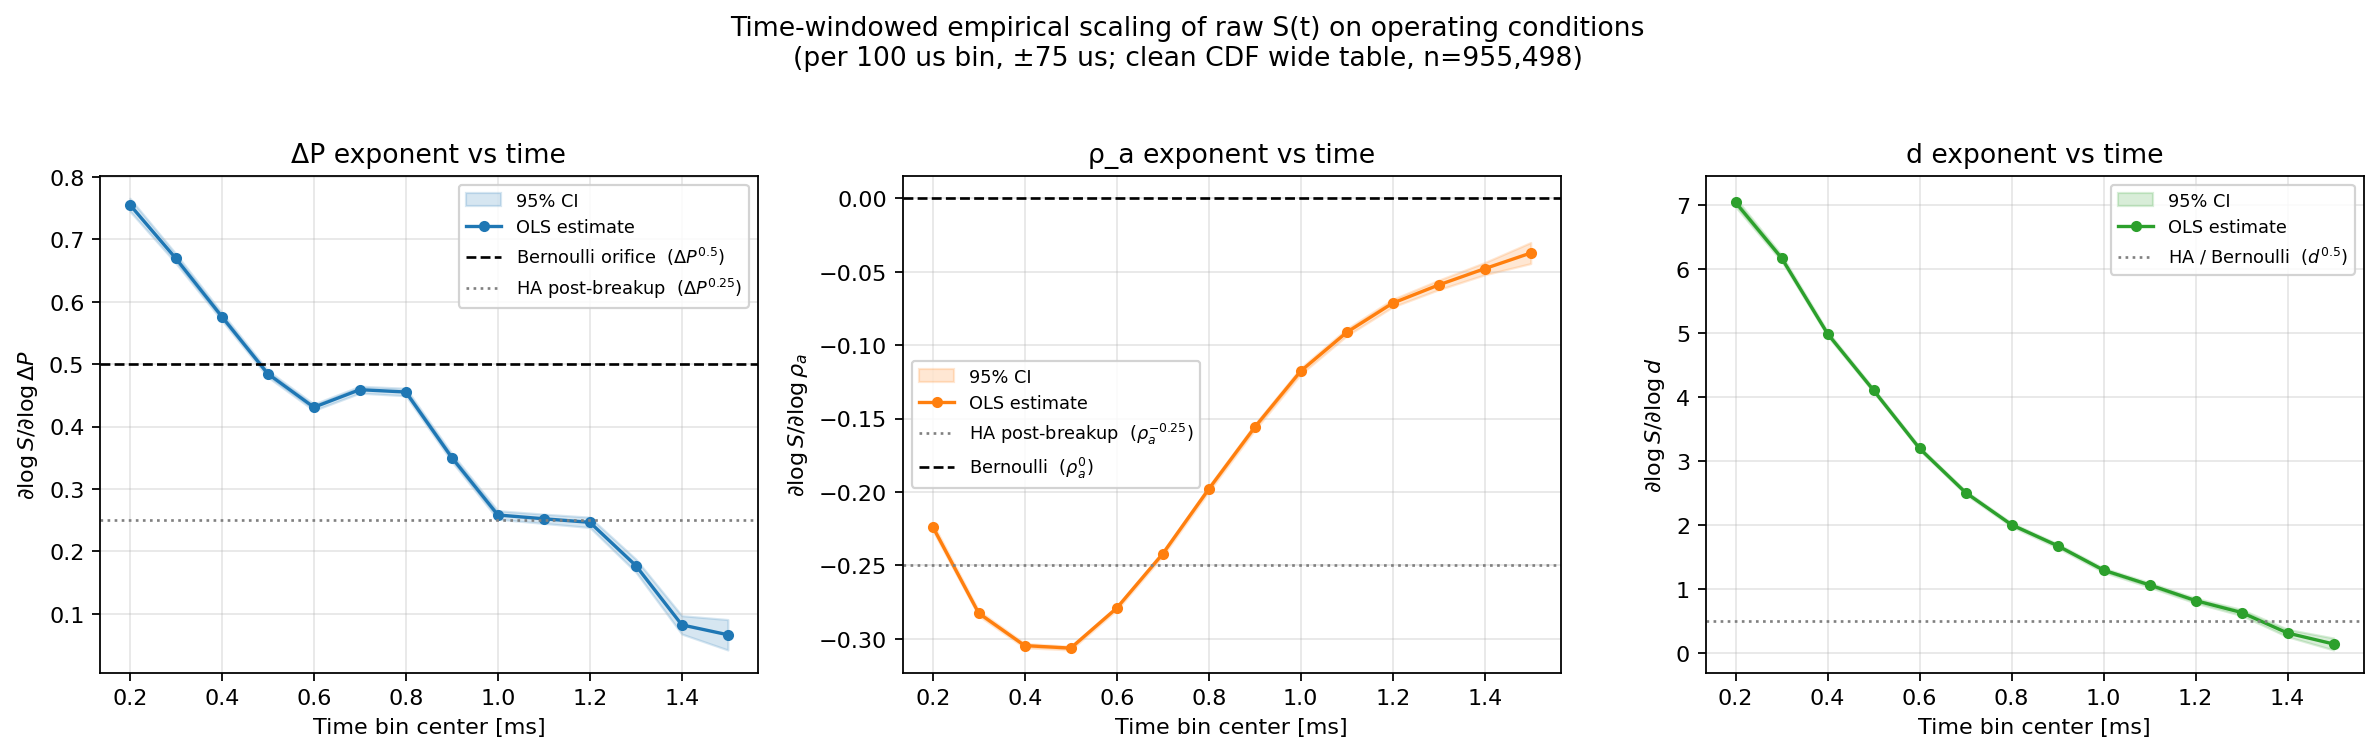
\includegraphics[width=0.94\linewidth,height=0.72\textheight,keepaspectratio]{time_windowed_exponents.png}

\vspace{0.15em}
\footnotesize
Regression target: \(S(t)\). Predictors: \(\log \Delta P\), \(\log \rho_a\), \(\log d_n\), fitted separately in time windows.

\src{MLP/synthetic_data/fit_diagnostics/time_windowed_exponent/time_windowed_exponents.png}
\end{frame}

\begin{frame}{Regime Transition in One Table}
\scriptsize
{\setlength{\tabcolsep}{3pt}
\begin{tabular}{R{0.08\linewidth}R{0.14\linewidth}R{0.14\linewidth}R{0.14\linewidth}R{0.11\linewidth}L{0.24\linewidth}}
\toprule
\(t\) ms & \(n\) & \(\Delta P\) exp. & \(\rho_a\) exp. & \(R^2\) & Interpretation \\
\midrule
0.20 & 161,533 & 0.755 & -0.224 & 0.32 & very early jet \\
0.40 & 142,590 & 0.576 & -0.305 & 0.60 & approaching orifice scale \\
\good{0.50} & 124,526 & \good{0.484} & -0.306 & \good{0.68} & \good{Bernoulli \(0.5\)} \\
0.70 & 81,230 & 0.459 & -0.242 & 0.57 & transition \\
\good{1.00} & 33,258 & \good{0.258} & -0.118 & 0.30 & \good{HA \(0.25\)} \\
1.20 & 12,314 & 0.247 & -0.071 & 0.30 & late asymptote \\
1.50 & 637 & 0.067 & -0.037 & 0.21 & pressure influence fades \\
\bottomrule
\end{tabular}
}

\vspace{0.5em}
\small
\textbf{Readout:} the data cross the Bernoulli \(\Delta P^{0.5}\) value around \SI{0.5}{ms} and the HA \(\Delta P^{0.25}\) value around \SI{1.0}{ms}. The model's representative mass lies closer to the transitional \(0.5\)--\SI{0.8}{ms} region than to a purely late-time asymptote.

\vfill{\tiny\textcolor{gray!75!black}{Source: slide asset CSV copied from time-windowed exponent diagnostics.}}
\end{frame}

\begin{frame}{Why \(0.5\), Not \(0.25\), \(0.7\), or \(1.0\)?}
\small
\begin{block}{Why not stay at HA \(0.25\)?}
HA is not wrong; it appears cleanly near \(t\approx\SI{1.0}{ms}\). The issue is applicability: the \(0\)--\SI{5}{ms} representative training mass is dominated by earlier transitional penetration, where \(\Delta P\) sensitivity is closer to \(0.5\).
\end{block}

\begin{block}{Why not use the earliest \(0.7\)--\(0.8\) exponent?}
The \(t=\SI{0.2}{ms}\) window has lower \(R^2\) and corresponds to onset / early-jet behavior handled by time features and Stage-3 onset refinement. \(A\)-scale is a per-condition length divisor, not a separate onset model.
\end{block}

\begin{block}{Physical interpretation}
\(\Delta P^{0.5}\) is the Bernoulli orifice velocity scale. The empirical result says the measured window still carries strong orifice-momentum imprint before the HA entrainment asymptote takes over.
\end{block}
\end{frame}

\begin{frame}{Computing $A$ from the Test Matrix}
\textbf{Per curve, $A$ is determined entirely from the operating point:}
\begin{itemize}
  \item $d_n$ from \texttt{nozzle\_properties.diameter\_mm} in the test matrix JSON
  \item $\Delta P=P_{\mathrm{inj}}-P_{\mathrm{ch}}$ from the per-row pressures
  \item $\rho_a$ from the linear law $\rho_a=\SI{5}{kg/m^3}\times P_{\mathrm{ch}}/\SI{4.42}{bar}$, calibrated against the explicit \texttt{chamber\_density\_kg\_per\_m3} entries provided for Nozzle1--8
\end{itemize}

\vspace{0.2em}
\[
\boxed{A_{\mathrm{scale}}=\Delta P^{0.5}\rho_a^{-0.25}\sqrt{d_n}}
\]

\vspace{0.4em}
\textbf{Implementation reference:}
\begin{itemize}
  \item \texttt{build\_canonical\_feature\_table} computes \texttt{delta\_pressure\_bar\_phys}, \texttt{ambient\_density\_kg\_m3}, \texttt{A\_scale}, and \texttt{log\_A}
  \item current code uses \texttt{np.power(delta\_pressure\_bar\_phys, 0.5)} in both training and inference paths
  \item Nozzle0 and Nozzle1--8 share the same canonicalization, so all datasets use one consistent $A$
\end{itemize}
\end{frame}

\begin{frame}{New Feature Set}
\textbf{Removed (4 sparse direct features):}
\[
\{\,d_n,\;\log P_{\mathrm{inj}},\;\log P_{\mathrm{ch}},\;\log\Delta P\,\}
\]

\textbf{Two variants are exposed in \texttt{FEATURE\_COLUMNS\_BY\_VARIANT}:}
\begin{itemize}
  \item \texttt{a\_only} (5 features):
  \[
  [\text{time}_{\mathrm{norm}},\;\theta_{\mathrm{tilt},z},\;n_{\mathrm{plumes},z},\;t_{i,z},\;P_{\mathrm{cb},z}]
  \]
  $A$ never enters as an input; it only acts as a divisor on the target.
  \item \texttt{a\_plus\_log\_a} (6 features):
  \[
  [\text{time}_{\mathrm{norm}},\;\theta_{\mathrm{tilt},z},\;n_{\mathrm{plumes},z},\;t_{i,z},\;P_{\mathrm{cb},z},\;\log A_z]
  \]
  $A$ also appears once as a one-dimensional residual axis.
\end{itemize}

\textbf{Why two variants:} \texttt{a\_only} is the strongest commitment to the data-supported transitional scaling. \texttt{a\_plus\_log\_a} lets the network express residual dependence on the scaling group as a single normalized axis instead of four sparse axes.
\end{frame}

\begin{frame}{Target Reparameterization}
\textbf{v1:} the network predicted $\mu(t)$ and $\log\sigma^2(t)$ on the physical penetration $S(t)$ in mm.

\vspace{0.3em}
\textbf{v2:} the network predicts the same two heads on the non-dimensional target
\[
\hat S(t)\;=\;S(t)/A,\qquad
\hat\sigma^2(t)\;=\;\sigma^2(t)/A^{2}.
\]
At inference, the physical mean and standard deviation are recovered exactly by
\[
\mu_S(t)\;=\;A\,\hat\mu(t),\qquad
\sigma_S(t)\;=\;A\,\hat\sigma(t).
\]

\vspace{0.3em}
\textbf{Implementation reference:} \texttt{PenetrationDataset} stores \texttt{target\_scaled = penetration / A\_scale} per row. The Stage-1 MSE and Stage-2 NLL objectives in \texttt{engineered\_feature\_common} consume \texttt{target\_scaled} directly, while \texttt{toy\_inference\_from\_run} multiplies the predicted mean and std by \texttt{A\_scale} when reporting in millimetres.
\end{frame}

\begin{frame}{Why This Should Help the Sparse-Feature Pathology}
\textbf{Mechanism:} the four sparse axes that produced spurious curvature in v1 are no longer free inputs. Their main effect is expressed through one analytic factor $A$ whose pressure exponent is selected by time-windowed data evidence rather than learned freely from a sparse grid.

\vspace{0.4em}
\textbf{Expected consequences:}
\begin{itemize}
  \item $\partial\mu_S/\partial d_n$ inherits the closed-form $d_n^{1/2}$ shape; the network has fewer degrees of freedom to invent oscillations along $d_n$
  \item $\partial\mu_S/\partial P_{\mathrm{inj}}$, $\partial\mu_S/\partial P_{\mathrm{ch}}$ inherit the closed-form \(\Delta P^{0.5}\rho_a^{-0.25}\) shape, with positive \(\Delta P\) sensitivity by construction
  \item all remaining learning capacity is spent on the dense, well-supported axes (time, tilt, plumes, injection duration, control backpressure)
\end{itemize}

\vspace{0.3em}
\textbf{Honest caveat:} this only helps if the selected scaling actually collapses the trajectories on the present data. That is why collapse checks and the \(\Delta P^{0.25}\) vs \(\Delta P^{0.5}\) ablation are part of the evidence chain.
\end{frame}

\begin{frame}{Empirical Outcome of the Exponent Change}
\small
\begin{block}{In-pipeline 5-seed result}
Changing \(A_{\mathrm{scale}}\) from \(\Delta P^{0.25}\) to \(\Delta P^{0.5}\) improved the mode-C 5-seed in-pipeline RMSE from \SI{10.72}{mm} to \SI{8.92}{mm}, a \good{16.8\% reduction}. Coverage also moved closer to target: 1\(\sigma\) from 0.497 to 0.654 and 2\(\sigma\) from 0.911 to 0.966.
\end{block}

\begin{block}{External clean diagnostic}
On the \num{795561}-point external clean protocol, the \(\Delta P^{0.5}\) Stage-3 MLP reached \good{RMSE \SI{6.211}{mm} \(\pm\) \SI{0.283}{mm}} over five seeds, compared with \SI{6.696}{mm} for the old \(\Delta P^{0.25}\) seed-42 model.
\end{block}

\begin{block}{Baseline context}
The same external comparison gives RMSE \SI{9.974}{mm} for calibrated Hiroyasu--Arai, \SI{8.840}{mm} for Naber--Siebers delay, and \SI{6.898}{mm} for sparse heteroscedastic GP.
\end{block}

\src{Thesis/generated/baseline_comparison_20260509/headline_comparison.csv}
\end{frame}

\begin{frame}{Pretrain Collapse Check}
Before any optimization, \texttt{run\_pretrain\_collapse\_check} reconstructs the representative trajectories from the four fitted constants, divides each by its own $A$, and tests whether
\[
\hat S(t)\;\approx\;\text{function of the remaining (dense) features only}.
\]

\vspace{0.3em}
\textbf{What it produces:}
\begin{itemize}
  \item per-time-slice variance of $\hat S(t)$ versus the original $S(t)$
  \item a linear regression $R^{2}$ of $\hat S(t)$ on the kept features
  \item a binary \texttt{passed} flag, surfaced in the run directory
\end{itemize}

\vspace{0.3em}
\textbf{Role in the pipeline:} if the precheck fails, training aborts unless \texttt{--allow-failed-precheck} is passed. This makes the physical assumption \emph{falsifiable} on the actual dataset rather than asserted.
\end{frame}

\begin{frame}{Collapse Metrics: What They Mean}
\small
\begin{block}{Collapse ratio}
\footnotesize
For each sampled time, the diagnostic compares the raw cross-condition spread with the
\(A\)-scaled spread:
\[
r_{\mathrm{collapse}}(t)=
\frac{\operatorname{std}_j(S_j(t)/A_j)}{\operatorname{std}_j(S_j(t))}.
\]
Values below 1 mean the analytic scale has removed condition-to-condition variance;
smaller is better. The headline number is the median over \(t\geq\SI{0.5}{ms}\).
\end{block}

\begin{block}{Sparse-feature \(R^2\)}
\footnotesize
A linear model tries to recover either \(S(t)\) or \(S(t)/A\) from only the sparse
axes \((d_n,P_{\mathrm{inj}},P_{\mathrm{ch}})\). If the scaled target still has high
\(R^2\), the divisor failed to remove the sparse axes. A successful collapse drives
\(R^2_{\mathrm{scaled}}/R^2_{\mathrm{physical}}\) downward.
\end{block}
\end{frame}

\begin{frame}{Collapse Evidence: \(\Delta P^{0.25}\) vs \(\Delta P^{0.5}\)}
\small
\begin{center}
\begin{tabular}{L{0.44\linewidth}R{0.19\linewidth}R{0.19\linewidth}}
\toprule
Diagnostic & \(\Delta P^{0.25}\) & \(\Delta P^{0.5}\) \\
\midrule
Median post-\SI{0.5}{ms} collapse ratio & 0.378 & \good{0.057} \\
Mean sparse \(R^2\), physical target & 0.416 & 0.416 \\
Mean sparse \(R^2\), scaled target & 0.054 & \good{0.023} \\
Scaled/physical sparse \(R^2\) ratio & 0.130 & \good{0.055} \\
All post-\SI{0.5}{ms} ratios \(<1\) & true & true \\
Pretrain check passed & true & true \\
\bottomrule
\end{tabular}
\end{center}

\vspace{0.35em}
\footnotesize
\textbf{Readout:} both exponents are admissible in the weak pass/fail sense, but
\(\Delta P^{0.5}\) removes far more cross-condition spread and leaves less residual
linear explainability in the sparse pressure/diameter axes. This is the pre-training
diagnostic counterpart to the post-training RMSE ablation.

\src{MLP/synthetic_data/fit_diagnostics/delta_p_exponent_collapse/comparison_summary.csv}
\end{frame}

\begin{frame}{Collapse Plots: Visual Check}
\begin{columns}[T,onlytextwidth]
\begin{column}{0.49\linewidth}
\centering
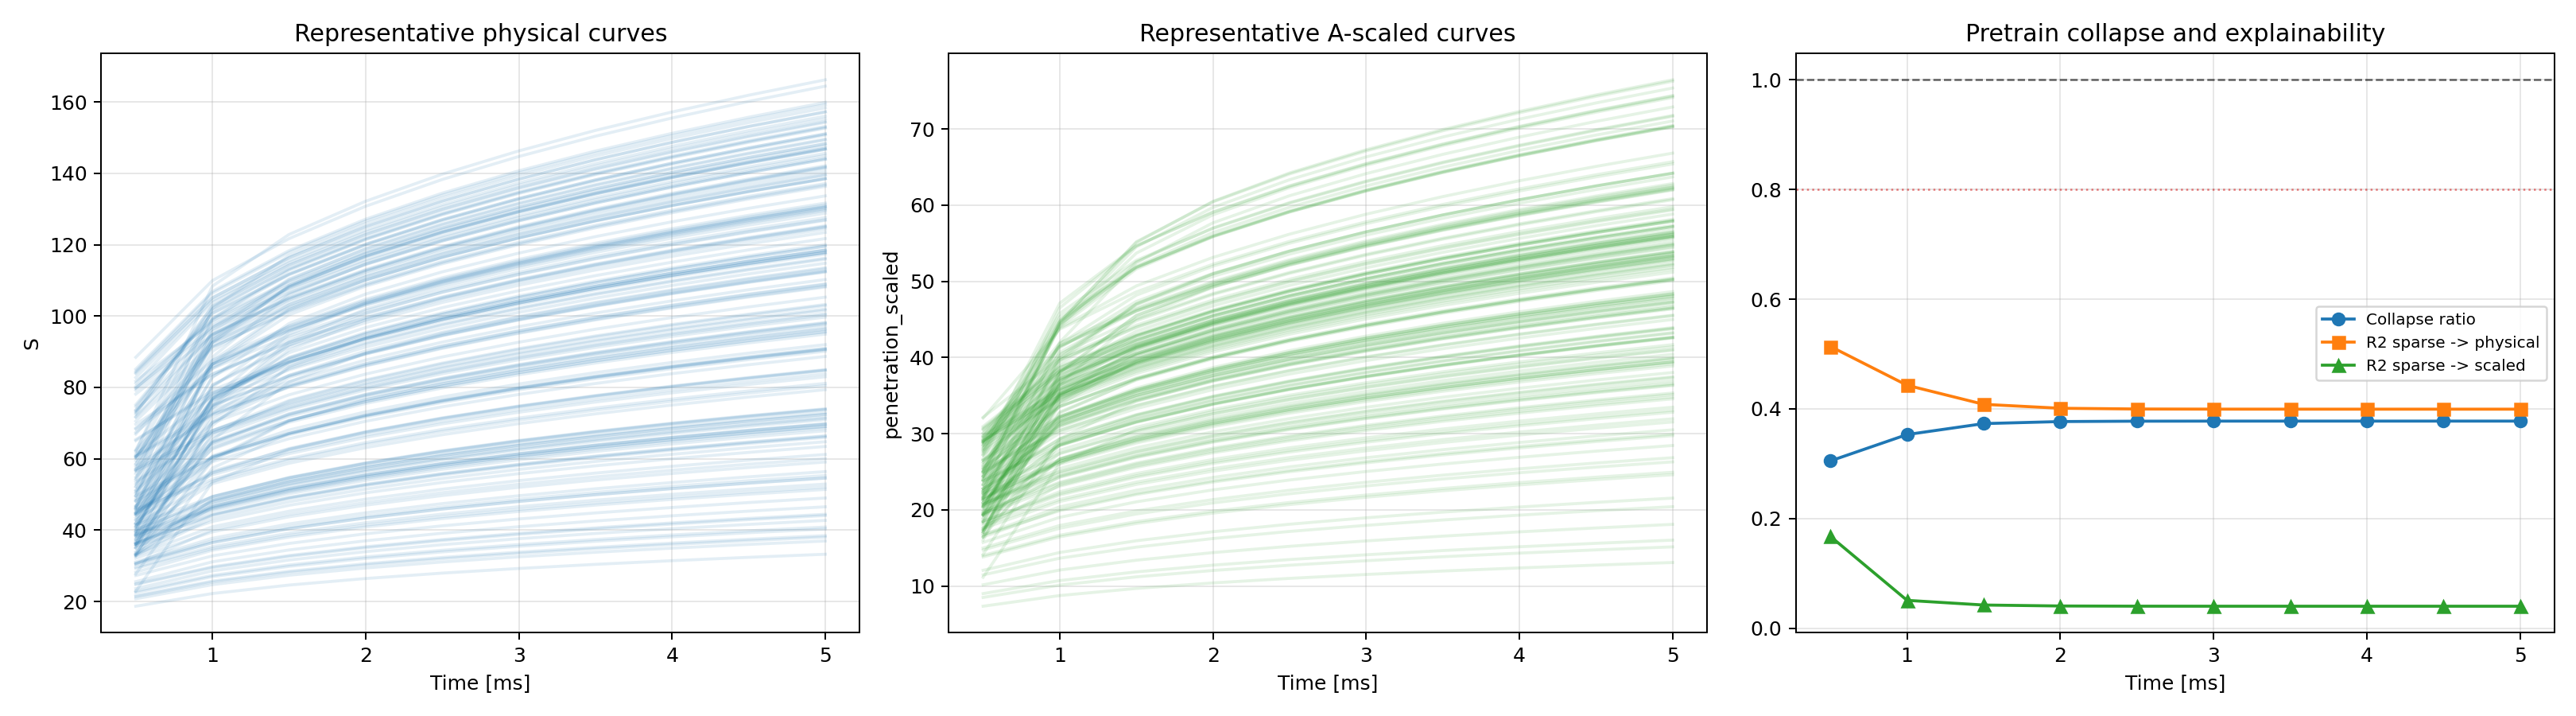
\includegraphics[width=\linewidth,height=0.68\textheight,keepaspectratio]{collapse_dp_exp_0p25.png}

\vspace{0.1em}
\footnotesize \(\Delta P^{0.25}\): valid but leaves visible residual spread.
\end{column}
\begin{column}{0.49\linewidth}
\centering
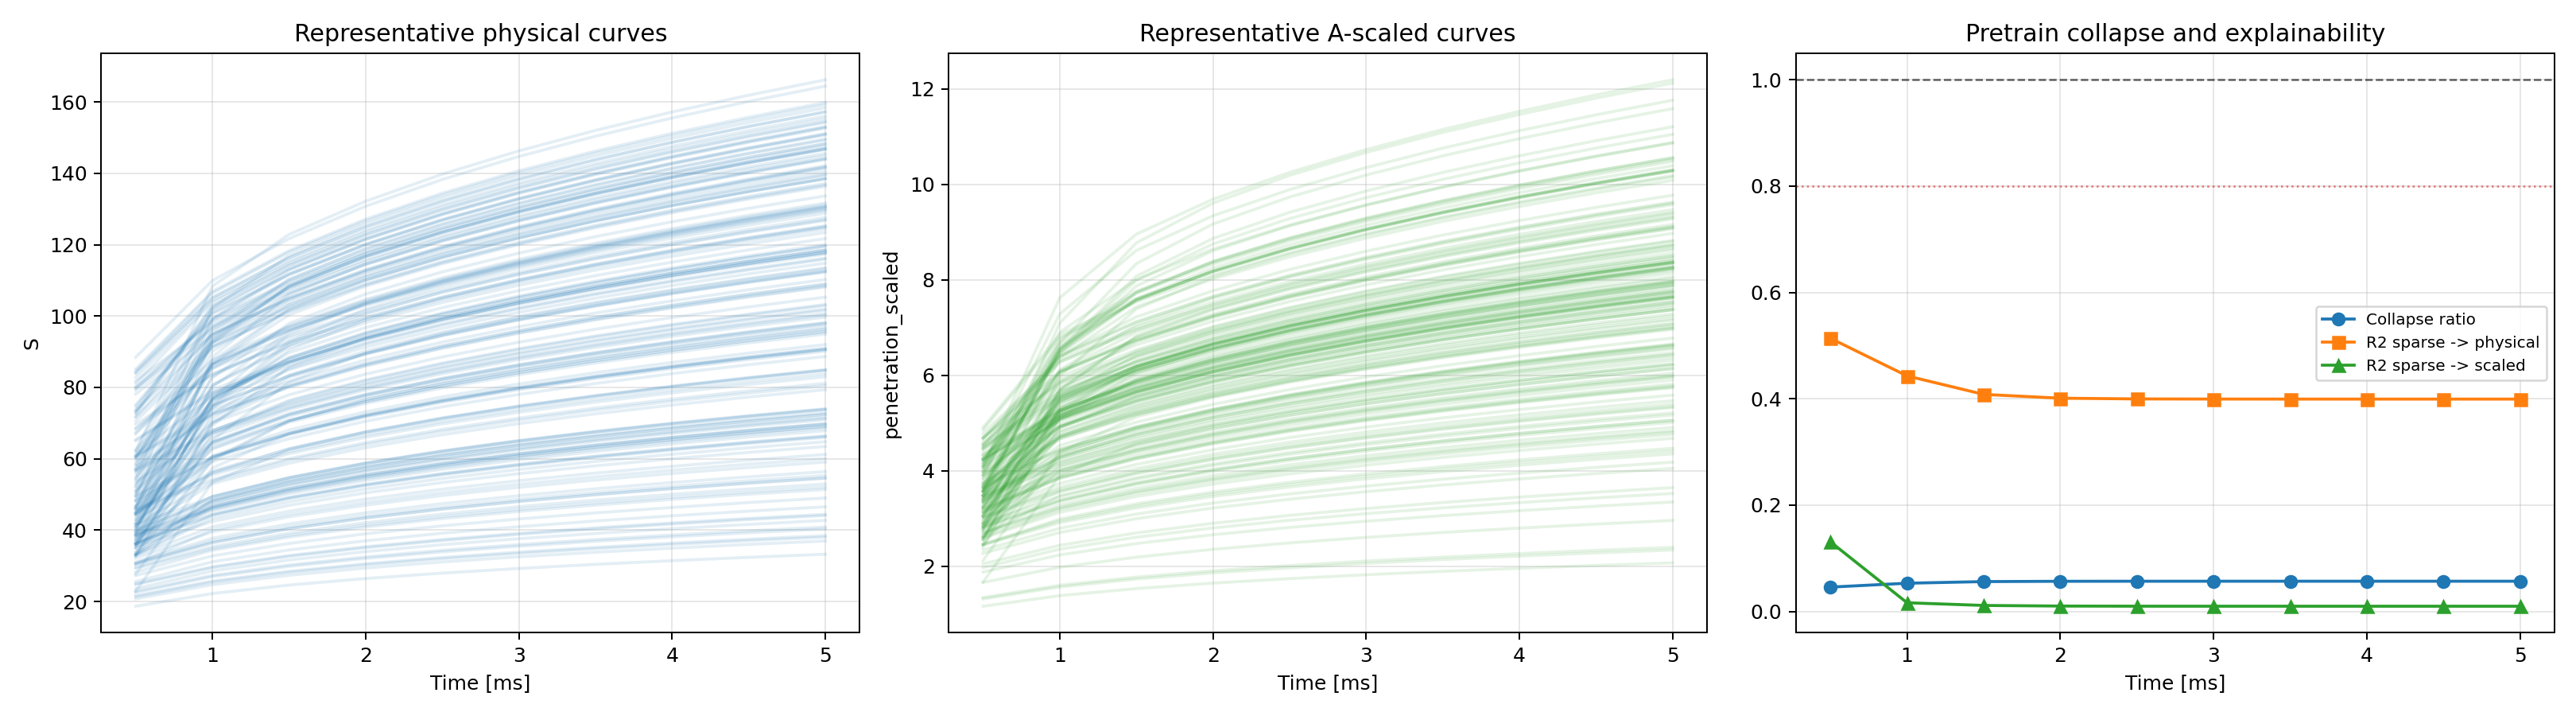
\includegraphics[width=\linewidth,height=0.68\textheight,keepaspectratio]{collapse_dp_exp_0p50.png}

\vspace{0.1em}
\footnotesize \(\Delta P^{0.5}\): tighter scaled trajectories and lower sparse \(R^2\).
\end{column}
\end{columns}

\src{MLP/synthetic_data/fit_diagnostics/delta_p_exponent_collapse/}
\end{frame}

\begin{frame}{Other Pipeline Changes}
\small
\textbf{Group-aware splits.} \texttt{assign\_splits\_by\_group} assigns whole \texttt{sample\_group\_id} groups to train/val/test instead of permuting individual rows.

\vspace{0.3em}
\textbf{Stage-1 / Stage-2 driver split.} Stage 2 warm-starts from a Stage-1 engineered run directory and reuses its scaler state, so the variant choice and the \(A\)-scaling remain identical between stages.

\vspace{0.3em}
\textbf{Loss objectives.} Stage-1 MSE and Stage-2 NLL consume \(S/A\). Monotonicity and post-transient concavity priors are applied on \(\hat\mu(t)\), then mapped back to millimetres by multiplying by \(A\).

\vspace{0.3em}
\textbf{Inference path.} Engineered runs canonicalize raw inputs through the same \(\rho_a\), \(\Delta P\), \(A\) pipeline used in training and rescale predicted mean/std by \(A\) before plotting.
\end{frame}

\begin{frame}{Engineering Takeaway}
\footnotesize
\textbf{What v3 commits to:}
\begin{itemize}
\setlength{\itemsep}{0.12em}
  \item the pressure/ambient/nozzle group is still treated as a hard divisor, not a soft regularizer
  \item the pressure exponent is now \(\Delta P^{0.5}\), supported by time-windowed regression in the dominant transitional regime
  \item the HA \(\Delta P^{0.25}\) exponent is retained as the late-time asymptotic interpretation, not rejected
  \item the network is no longer asked to learn a continuous law over a $6$-point diameter grid or a $4$-point pressure grid
  \item the resulting model is falsifiable: if the collapse check or held-out ablation fails, the selected exponent is wrong on this dataset
\end{itemize}

\vspace{0.15em}
\textbf{Completed evidence now available:}
\begin{itemize}
\setlength{\itemsep}{0.12em}
  \item report the time-windowed exponent figure as the physical justification for \(0.5\)
  \item report the collapse-ratio comparison as the pre-training diagnostic justification
  \item report the 5-seed \(\Delta P^{0.25}\) vs \(\Delta P^{0.5}\) ablation as the ML justification
  \item keep the diameter exponent caveat: early \(d_n\) exponents are confounded by nozzle family and limited diameter support
\end{itemize}
\end{frame}

\begin{frame}{Data Sources for Thesis Extraction}
\small
\begin{tabular}{L{0.28\linewidth}L{0.64\linewidth}}
\toprule
Item & Path \\
\midrule
Time-windowed regression CSV &
\scriptsize\url{MLP/synthetic_data/fit_diagnostics/time_windowed_exponent/time_windowed_scaling_regression.csv} \\
Regime-transition figure &
\scriptsize\url{MLP/synthetic_data/fit_diagnostics/time_windowed_exponent/time_windowed_exponents.png} \\
Current \(A_{\mathrm{scale}}\) implementation &
\scriptsize\url{MLP/MLP_training/engineered_feature_common.py} lines around \texttt{A\_scale} construction \\
Baseline / GP comparison snapshot &
\scriptsize\url{Thesis/generated/baseline_comparison_20260509/headline_comparison.csv} \\
Collapse comparison summary &
\scriptsize\url{MLP/synthetic_data/fit_diagnostics/delta_p_exponent_collapse/comparison_summary.csv} \\
Slide-local frozen copies &
\scriptsize\url{Thesis/slides/slides_engineered_feature/assets/} \\
\bottomrule
\end{tabular}

\vspace{0.6em}
\textbf{Thesis sentence to extract:} Time-windowed log--log regression shows the empirical \(\Delta P\) exponent decaying from 0.76 at \SI{0.2}{ms} to 0.26 at \SI{1.0}{ms}, crossing the Bernoulli \(0.5\) scale around \SI{0.5}{ms} and the HA \(0.25\) asymptote around \SI{1.0}{ms}. This motivates using \(\Delta P^{0.5}\) in \(A_{\mathrm{scale}}\) for the dominant transitional data regime.
\end{frame}

\end{document}
